\documentclass[12pt]{article}
\usepackage[utf8]{inputenc}
\usepackage[english]{babel}
\usepackage{graphicx}
\usepackage{float}
\usepackage{amsmath}
\usepackage{xcolor}
\usepackage{enumitem}
\usepackage{titlesec}
\usepackage{amssymb}
\usepackage{caption}

\title{Homework 2}
\author{Leonard David Vivas Dallos \\ Mariana Valencia Cubillos \\ Samuel Mira Álvarez}
\date{September 13, 2023}

\begin{document}

\maketitle

\textbf{\textit{Assignment:}} Write solutions for exercises/problems
\begin{equation*}
    1, 2(e, f, g), 3, 4, 6, 8(b, c).
\end{equation*}

\tableofcontents

\section{Exercise 1: \textit{Operations on languages}}

Prove that for all languages A, B, and C:
\begin{enumerate}
    \item $(A \cup B)^* = (A^* \text{ • } B^* )^*$.
    \item (ERICKSON, EX 2.1 (f)) If $A \cdot B = B \cdot C$, then $A^* \cdot B = B \cdot C^* = A^* \cdot B \cdot C^*$.
\end{enumerate}

\textit{Hint:} A recursive definition of $A^*: w \in A^*$ if either $w = \varepsilon$ or $w = xy$ where $x \in A$ and $y \in A^*$. Alternatively, $A^* = \bigcup_{k=0}^{\infty} A^k$.

\subsection{Proof}
Let $A, B$ be arbitrary languages. Let's see that
\begin{equation*}
    (A \cup B)^* = (A^* \text{ • } B^* )^*
\end{equation*}

$"\subseteq"$

Let $w \in L((A \cup B)^*)$ an arbitrary string. Then, $w$ is of the form
\begin{equation*}
    w_1 \cdot w_2 \cdot \dotsb \cdot w_n
\end{equation*}
 where each $w_i \in L(A) \cup L(B)$. Now, for each one of the $w_i$ in $w$ we have two options:
 \begin{enumerate}
     \item $w_i \in L(A)$. If this holds, then $w_i = w_i \cdot \varepsilon$ which belongs to $L(A^*B^*)$.
     \item $w_i \in L(B)$. If this holds, then $w_i = \varepsilon \cdot w_i$ which belongs to $L(A^*B^*)$.
 \end{enumerate}
 Now, as each $w_i \in L(A^*B^*)$, then, $w \in L((A^*B^*)^*)$
 As $w$ is an arbitrary string, $L((A \cup B)^*) \subseteq L((A^*B^*)^*)$

 $"\supseteq"$

 Let $w \in L((A^*B^*)^*)$ an arbitrary string. Then, $w$ is of the form
 \begin{equation*}
     w_1 \cdot w_2 \cdot \dotsb \cdot w_n
 \end{equation*}
 where each $w_i \in L(A^*B^*)$. Now, each one of the $w_i$ can be written as:
 \begin{equation*}
     v_1 \cdot v_2 \cdot \dotsb \cdot v_r \cdot u_1 \cdot u_2 \cdot \dotsb \cdot u_s
 \end{equation*}
 where $v_j \in L(A)$, $u_k \in L(B)$ and $r, s \geq 0$

 It is clear that $L(A) \subseteq L(A) \cup L(B)$ and $L(B) \subseteq L(A) \cup L(B)$. Then, $v_j \in L(A) \cup L(B)$ and $u_k \in L(A) \cup L(B)$. As $v_j$ and $u_k$ belongs to $w_i$, we have that $w_i \in L(A) \cup L(B)$.
 As this holds for each $i$, $w \in (L(A) \cup L(B))^*$, ie, $w \in L((A \cup B)^*)$. So, $L((A^*B^*)^*) \subseteq L((A \cup B)^*)$

 Then, $L((A \cup B)^*) = L((A^*B^*)^*) \Longleftrightarrow (A \cup B)^* = (A^* \text{ • } B^* )^*$

 \subsection{Proof}

 Let $A, B, C$ be languages such that $A \cdot B = B \cdot C$ Let's see that $A^* \cdot B = B \cdot C^* = A^* \cdot B \cdot C^*$
 We know that $w \in A^*$ if $w = \varepsilon$ or $w = xy$ with $x \in A$ and $y \in A^*$
 \begin{equation*}
     A^* = \bigcup_{k=0}^{\infty} A^k
 \end{equation*}
By induction over $k$

\textbf{Base Case:}
Let $k=0$. Then $w = \varepsilon$
\begin{equation*}
    A^0 \cdot B = \varepsilon \cdot B = B \cdot \varepsilon = B \cdot C^0
\end{equation*}

\textbf{Inductive Hypothesis (IH):}
Assume that for $k > 0$, if $A \cdot B = B \cdot C$, then $A^{k-1} \cdot B = B \cdot C^{k-1}$

\textbf{Inductive Step:}
Let's see the $k$ case, i.e. let's see what is $A^k \cdot B$
\begin{flalign*}
    A^k \cdot B &= (A \cdot A^{k-1}) \cdot B \quad \text{(By definition)} \\
    &=A \cdot (A^{k-1} \cdot B) \quad \text{(By associative property)}  \\
    &=A \cdot (B \cdot C^{k-1}) \quad \text{(By IH)} \\
    &=(A \cdot B) \cdot C^{k-1} \quad \text{(By associative property)} \\
    &=(B \cdot C) \cdot C^{k-1} \quad \text{(By hypothesis condition)} \\
    &=B \cdot (C \cdot C^{k-1}) \quad \text{(By associative property)} \\
    &=B \cdot C^k \quad \text{(By definition)}
\end{flalign*}

Hence, for $k > 0$, if $A \cdot B = B \cdot C$, then $A^k \cdot B = B \cdot C^k$.

Since the recursive definition of $A^*$, we have
\begin{flalign*}
    A^* \cdot B &= \left(\bigcup_{k=0}^{\infty} A^k\right) \cdot B \quad \text{(By recursive definition)} \\
    &= \bigcup_{k=0}^{\infty} (A^k \cdot B) \quad \text{(By properties)} \\
    &= \bigcup_{k=0}^{\infty} (B \cdot C^k) \quad \text{(By the result of induction)} \\
    &= B \cdot \bigcup_{k=0}^{\infty} C^k \quad \text{(By properties)} \\
    &= B \cdot C^* \quad \text{(By recursive definition)}
\end{flalign*}

Then, it was proven that $A^* \cdot B = B \cdot C^*$ if $A \cdot B = B \cdot A$. Now, let's see that $A^* \cdot B \cdot C^* = B \cdot C^*$
\begin{flalign*}
    A^* \cdot B \cdot C^* &= (A^* \cdot B) \cdot C^* \quad \text{(By associative property)} \\
    &= (B \cdot C^*) \cdot C^* \quad \text{(By result proven before)} \\
    &= B \cdot (C^* \cdot C^*) \quad \text{(By associative property)} \\
    &= B \cdot C^* \quad \text{(By recursive definition)}
\end{flalign*}

Then, it was proven that if $A \cdot B = B \cdot C$, $A^* \cdot B = B \cdot C^* = A^* \cdot B \cdot C^*$

\renewcommand{\thesubsection}{\thesection.\alph{subsection}}

\section{Exercise 2: \textit{DFA construction}}

For each of the following languages in $\{ 0, 1 \}^*$, describe a deterministic finite-state machine that accepts that language. Try to make it as simple as possible and argue that it is correct.

\begin{enumerate}
[label=\alph*), start=5]
    \item Every string whose reversal represents a number divisible by 7 in binary.
    \item Strings such that in every prefix, the number of $0$'s and the number of $1$'s differ by at most 3.
    \item Strings w such that $\binom{|w|}{2}mod6 = 4$
\end{enumerate}

\setcounter{subsection}{4}

\subsection{Proof} 

We need to build a DFA $N = (Q, \Sigma, \delta, q_0, F)$ .  

Since we are dealing with divisibility by 7, we will establish N with 7 states, each representing the remainder when performing division by 7. These states shall be denoted as \(q_0\), \(q_1\), \(q_2\), \(q_3\), \(q_4\), \(q_5\), and \(q_6\), where \(q_i\) is the remainder \(i\) resulting from the division by 7. 

The initial state will be \(q_0\) since the remainder is 0 when dividing an empty string (which represents 0) by 7. The accepting state will also be \(q_0\) because we aim to accept strings whose reversal represents a number divisible by 7, i.e., with a remainder of 0. 

We need to define the transition function \(\delta\) such that \(\delta(q_i, x) = q_j\), where \(x\) is the input symbol (0 or 1), and \(q_i\) and \(q_j\) represent the current and next states, respectively.

With this in mind, we can define $N = (Q, \Sigma, \delta, q_0, F)$ as follows:
\begin{enumerate}
\item $Q =  \{q_0, q_1, q_2, q_3, q_4, q_5, q_6\}$ 
\item $q_0$ will be the start state 
\item $F = \{q_0\}$
\item $\delta$ can be defined as follows:
  \[
\delta^*(q, w) =
\begin{cases}
q \text{ if } w = \epsilon  \\
\delta^*(\delta(q, a), x) \text{ if } w=xa \text{ and } a \in \Sigma
\end{cases}
\]
\end{enumerate}
\begin{table}[h]
\centering
\begin{tabular}{|c|c|c|}
\hline
\textbf{Current State} & \textbf{0}& \textbf{1}\\
\hline
$q_0$ & $q_0$ & $q_1$ \\
$q_1$ & $q_6$ & $q_2$ \\
$q_2$ & $q_5$ & $q_3$ \\
$q_3$ & $q_4$ & $q_0$ \\
$q_4$ & $q_3$ & $q_1$ \\
$q_5$ & $q_2$ & $q_6$ \\
$q_6$ & $q_4$ & $q_5$ \\
\hline
\end{tabular}
\caption{ Transition Function $\delta$ for the DFA N}
\end{table}

\begin{minipage}{\textwidth}
    \centering
    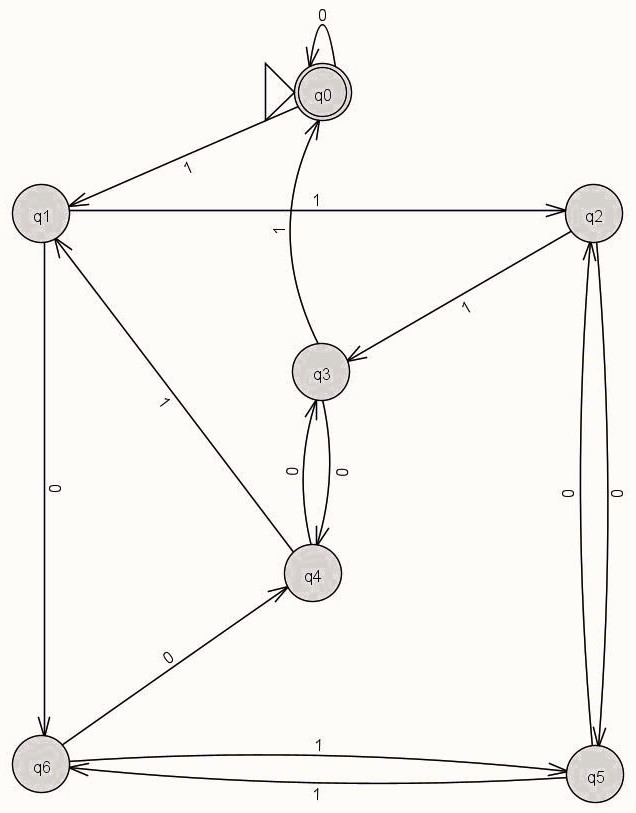
\includegraphics[width=0.5\textwidth]{Tarea 2 DFA 2.e.jpg}
    \captionof{figure}{DFA N representation}
    \label{DFA N}
\end{minipage}

\subsection{Proof} 

We need to build a DFA $N = (Q, \Sigma, \delta, q_0, F)$ .

We need to keep track of the difference between the number of 0s and the number of 1s in the string. Since the difference can be at most 3, we can have the following states:
\begin{itemize}
    \item $q_0$: the difference is 0
    \item $q_1$: one more 0 than 1
    \item $q_2$: two more 0s than 1s
    \item $q_3$: three more 0s than 1s
    \item $q_{-1}$: one more 1 than 0
    \item $q_{-2}$: two more 1s than 0s
    \item $q_{-3}$: three more 1s than 0s
    \item $q_O$: when the difference is more than 3 (out of range)

\end{itemize}

We can define $N = (Q, \Sigma, \delta, q_0, F)$ as follows:
\begin{enumerate}
\item $Q =  \{q_0, q_1, q_2, q_3, q_{-1}, q_{-2}, q_{-3}, q_O\}$
\item $q_0$ is the start state
\item $F = \{  q_0, q_1, q_2, q_3, q_{-1}, q_{-2}, q_{-3}\}$
\item $\delta$ is defined as 
\end{enumerate}
  \[
\delta^*(q, w) =
\begin{cases}
q \text{ if } w = \epsilon  \\
\delta^*(\delta(q, a), x) \text{ if } w=ax \text{ and } a \in \Sigma
\end{cases}
\]
\begin{table}[h]
\centering
\begin{tabular}{|c|c|c|}
\hline
\textbf{Current State} & \textbf{0}& \textbf{1}\\
\hline
$q_0$ & $q_1$& $q_{-1}$\\
$q_1$ & $q_2$& $q_0$\\
$q_2$ & $q_3$& $q_1$\\
 $q_3$& $q_O$&$q_2$\\
$q_{-1}$& $q_0$& $q_{-2}$\\
$q_{-2}$& $q_{-1}$& $q_{-3}$\\
$q_{-3}$& $q_{-2}$& $q_O$\\
$q_O$& $q_{-3}$& $q_3$\\
\hline
\end{tabular}
\caption{ Transition Function $\delta$ for the DFA N}
\end{table}

\begin{figure}
    \centering
    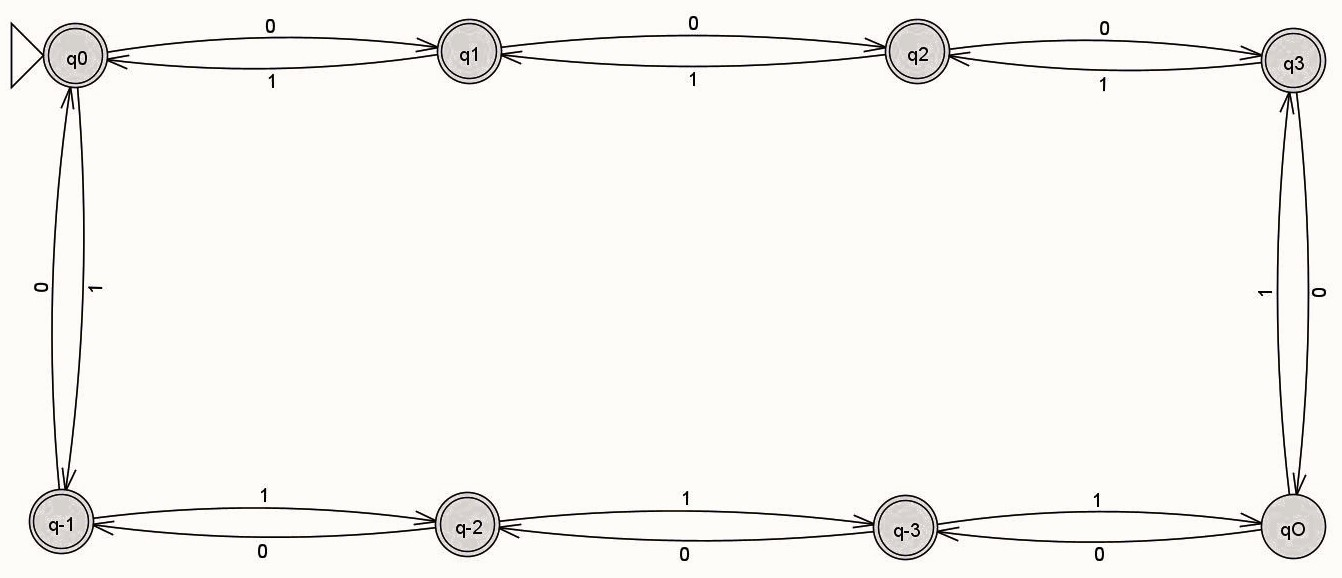
\includegraphics[width=0.75\linewidth]{Tarea 2 DFA 2.f.jpg}
    \caption{DFA N representation}
    \label{DFA N}
\end{figure}

\subsection{Proof} 

We need to construct a Deterministic Finite Automaton (DFA) $N = (Q, \Sigma, \delta, q_0, F)$.

The Non-deterministic Finite Automaton (NFA) must keep track of both $\binom{|w|}{2} \mod 6$ and $|x| \mod 6$, where $x$ represents the prefix of the input read so far. Therefore, the states of $N$ should be of the form $(\binom{|w|}{2} \mod 6, |x| \mod 6)$. Thus, we define $N$ as follows:

\begin{enumerate}
    \item $Q = \{0, 1, 2, 3, 4, 5, 6\} \times \{0, 1, 2, 3, 4, 5, 6\}$
    \item $(0, 0)$ is the initial state $q_0$.
    \item $F = \{(4, p) \mid p \in \{0, 1, 2, 3, 4, 5\}\}$
    \item $\delta = (q + p \mod 6, p + 1 \mod 6)$ for all $q \in Q$ and $p \in \{0, 1, 2, 3, 4, 5\}$, with $a \in \Sigma$. We can define $\delta$ in this way due to the identity $\binom{n+1}{2} = \binom{n}{2} + n$.
\end{enumerate}


\section{Exercise 3: \textit{NFA and DFA construction}}
\begin{enumerate}
[label=\alph*)]
    \item Give an NFA that accepts the language L over $\Sigma = \{ a, b, c \}$ that consists of strings with the string $w = aabaabcaaab$ as a suffix.
    \item Convert the NFA obtained into a DFA using the "subset construction" but including only those states in the construction that are reachable from the initial state. Is the DFA obtained of minimun size?
    \item Give an DFA that accepts the language that consists of string with either $w = aabaabacaab$ or $w' = baaba$ as suffix. Argue that your DFA is correct and that it is of minimun size (number of states).
\end{enumerate}

\subsection{NFA that accepts $w = aabaabcaaab$ as a suffix}
\begin{figure}[h]
    \centering
    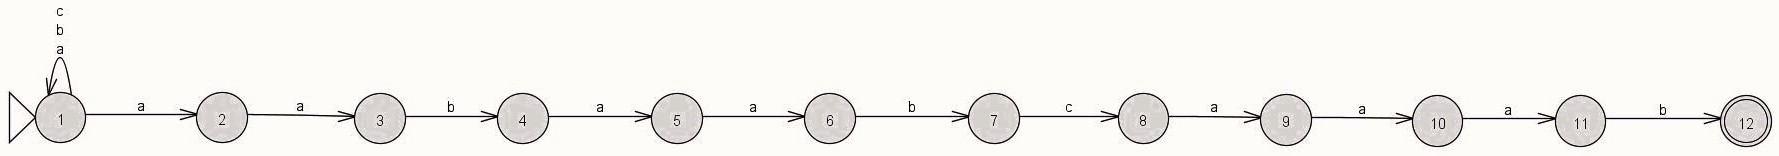
\includegraphics[width=1\linewidth]{Tarea 2 NFA 3.a.jpg}
    \caption{NFA that accepts $w = aabaabcaaab$ as a suffix}
    \label{NFA 1}
\end{figure}

\subsection{Conversion to DFA using "subset construction"}

\begin{center}
  \begin{tabular}{|c|c|c|c|}
    \hline
     & a & b & c \\
    \hline
    \textbf{In:} 1 & 1, 2 & 1 & 1 \\
    \hline
    2 & 3 &  & \\
    \hline
    3 &  & 4 & \\
    \hline
    4 & 5 &  & \\
    \hline
    5 & 6 &  & \\
    \hline
    6 &  & 7 & \\
    \hline
    7 &  &  & 8 \\
    \hline
    8 & 9 &  & \\
    \hline
    9 & 10 &  & \\
    \hline
    10 & 11 &  & \\
    \hline
    11 &  & 12 & \\
    \hline
    \textbf{Accept:} 12 &  &  & \\
    \hline
  \end{tabular}
  \captionof{table}{NFA Table}
\end{center}

\begin{center}
  \begin{tabular}{|c|c|c|c|c|}
    \hline
     & a & b & c & Notation\\
    \hline
    \textbf{In:} 1 & \{1, 2\} & 1 & 1 & $q_0$ \\
    \hline
    \{1, 2\} & \{1, 2, 3\} & 1 & 1 & $q_1$ \\
    \hline
    \{1, 2, 3\} & \{1, 2, 3\} & \{1, 4\} & 1 & $q_2$ \\
    \hline
    \{1, 4\} & \{1, 2, 5\} & 1 & 1 & $q_3$ \\
    \hline
    \{1, 2, 5\} & \{1, 2, 3, 6\} & 1 & 1 & $q_4$ \\
    \hline
    \{1, 2, 3, 6\} & \{1, 2, 3\} & \{1, 4, 7\} & 1 & $q_5$ \\
    \hline
    \{1, 4, 7\} & \{1, 2, 5\} & 1 & \{1, 8\} & $q_6$ \\
    \hline
    \{1, 8\} & \{1, 2, 9\} & 1 & 1 & $q_7$ \\
    \hline
    \{1, 2, 9\} & \{1, 2, 3, 10\} & 1 & 1 & $q_8$ \\
    \hline
    \{1, 2, 3, 10\} & \{1, 2, 3, 11\} & \{1, 4\} & 1 & $q_9$ \\
    \hline
    \{1, 2, 3, 11\} & \{1, 2, 3\} & \{1, 4, 12\} & 1 & $q_{10}$ \\
    \hline
    \textbf{Accept:} \{1, 4, 12\} & \{1, 2, 5\} & 1 & 1 & $q_{11}$ \\
    \hline
  \end{tabular}
  \captionof{table}{DFA Table}
\end{center}

\begin{figure}[h]
    \centering
    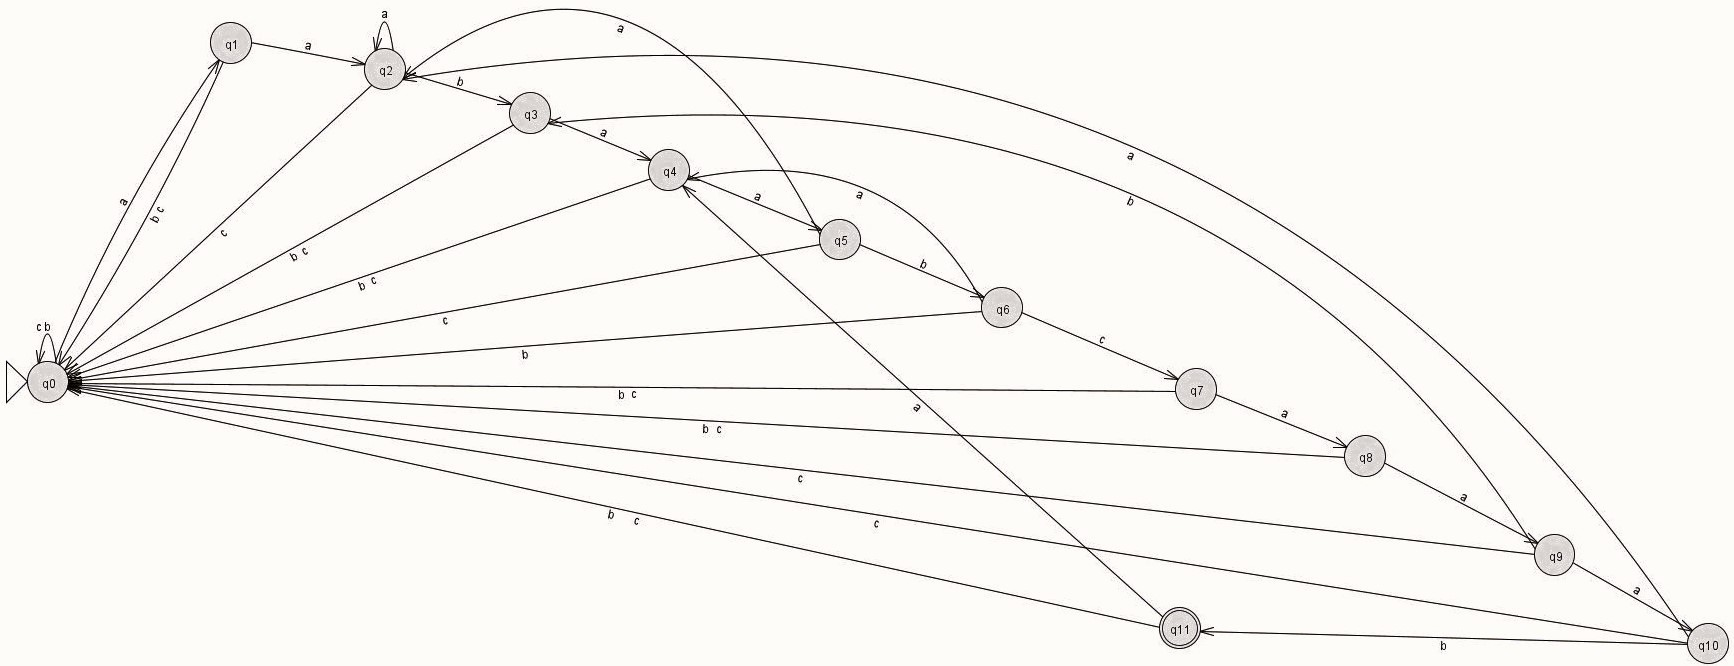
\includegraphics[width=1\linewidth]{Tarea 2 NFA 3.b.jpg}
    \caption{DFA that accepts $w = aabaabcaaab$ as a suffix}
    \label{DFA 1}
\end{figure}.

\subsection{DFA that accepts $w = aabaabacaab$ or $w' = baaba$ as suffix}

Let's build the requested DFA from an NFA. First of all, let's show the NFA that fulfills the request:

\begin{minipage}{\textwidth}
    \centering
    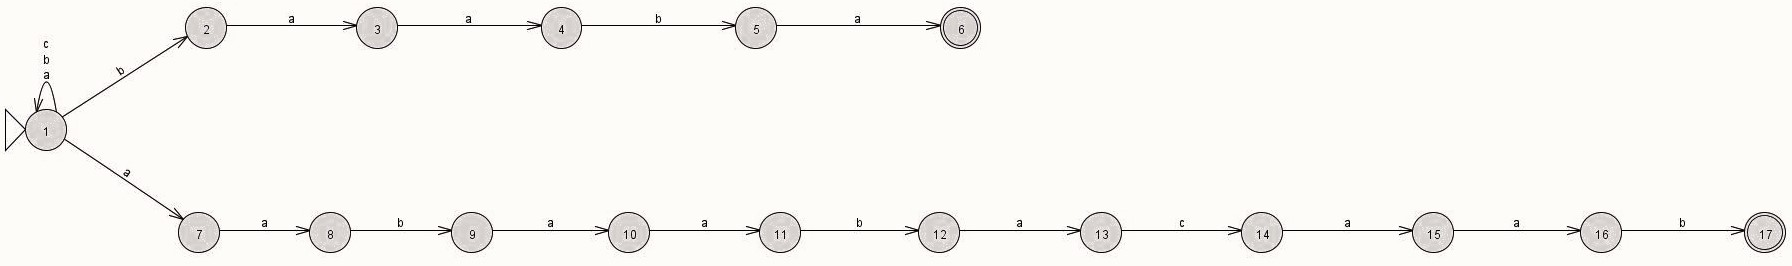
\includegraphics[width=1\textwidth]{Tarea 2 NFA 3.c.jpg}
    \captionof{figure}{NFA that accepts $w = aabaabacaab$ or $w' = baaba$ as suffix}
    \label{NFA 2}
\end{minipage}

Now, let's convert the NFA shown to an DFA using the subset construction

\begin{center}
  \begin{tabular}{|c|c|c|c|}
    \hline
     & a & b & c \\
    \hline
    \textbf{In:} 1 & 1, 7 & 1, 2 & 1 \\
    \hline
    2 & 3 &  & \\
    \hline
    3 & 4 &  & \\
    \hline
    4 &  & 5 & \\
    \hline
    5 & 6 &  & \\
    \hline
    \textbf{Accept:} 6&  &  & \\
    \hline
    7 & 8 &  & \\
    \hline
    8 &  & 9 & \\
    \hline
    9 & 10 &  & \\
    \hline
    10 & 11 &  & \\
    \hline
    11 &  & 12 & \\
    \hline
    12 & 13 &  & \\
    \hline
    13 &  &  & 14\\
    \hline
    14 &  15& & \\
    \hline
    15 &  16& & \\
    \hline
    16 &  & 17& \\
    \hline
    \textbf{Accept:} 17&  & & \\
    \hline
  \end{tabular}
  \captionof{table}{NFA Table}
\end{center}

\begin{center}
  \begin{tabular}{|c|c|c|c|c|}
    \hline
     & a & b & c & Notation\\
    \hline
    \textbf{In:} 1 & \{1, 7\} & \{1, 2\} & 1 & $q_0$ \\
    \hline
    \{1, 7\} & \{1, 7, 8\} & \{1, 2\} & 1 & $q_1$ \\
    \hline
    \{1, 2\} & \{1, 7, 3\} & \{1, 2\} & 1 & $q_2$ \\
    \hline
    \{1, 7, 8\} & \{1, 7, 8\} & \{1, 2, 9\} & 1 & $q_3$ \\
    \hline
    \{1, 7, 3\} & \{1, 4, 7, 8\} & \{1, 2\} & 1 & $q_4$ \\
    \hline
    \{1, 2, 9\} & \{1, 7, 3, 10\} & \{1, 2\} & 1 & $q_5$ \\
    \hline
    \{1, 4, 7, 8\} & \{1, 7, 8\} & \{1, 2, 5, 9\} & 1 & $q_6$ \\
    \hline
    \{1, 7, 3, 10\} & \{1, 7, 4, 8, 11\} & \{1, 2\} & 1 & $q_7$ \\
    \hline
    \{1, 2, 5, 9\} & \{1, 7, 3, 6, 10\} & \{1, 2\} & 1 & $q_8$ \\
    \hline
    \{1, 7, 4, 8, 11\} & \{1, 7, 8\} & \{1, 2, 5, 9, 12\} & 1 & $q_9$ \\
    \hline
    \textbf{Accept:} \{1, 7, 3, 6, 10\} & \{1, 7, 4, 8, 11\} & \{1, 2\} & 1 & $q_{10}$ \\
    \hline
    \{1, 2, 5, 9, 12\} & \{1, 7, 3, 6, 10, 13\} & \{1, 2\} & 1 & $q_{11}$ \\
    \hline
    \textbf{Accept:} \{1, 7, 3, 6, 10, 13\} & \{1, 7, 4, 8, 11\} & \{1, 2\} & \{1, 14\} & $q_{12}$ \\
    \hline
    \{1, 14\} & \{1, 7, 15\} & \{1, 2\} & 1 & $q_{13}$ \\
    \hline
    \{1, 7, 15\} & \{1, 7, 8, 16\} & \{1, 2\} & 1 & $q_{14}$ \\
    \hline
    \{1, 7, 8, 16\} & \{1, 7, 8\} & \{1, 2, 9, 17\} & 1 & $q_{15}$ \\
    \hline
    \textbf{Accept:} \{1, 2, 9, 17\} & \{1, 7, 3\} & \{1, 2\} & 1 & $q_{16}$ \\
    \hline
  \end{tabular}
  \captionof{table}{DFA Table}
\end{center}

With the table above, we can easily show the DFA.

\begin{minipage}{\textwidth}
    \centering
    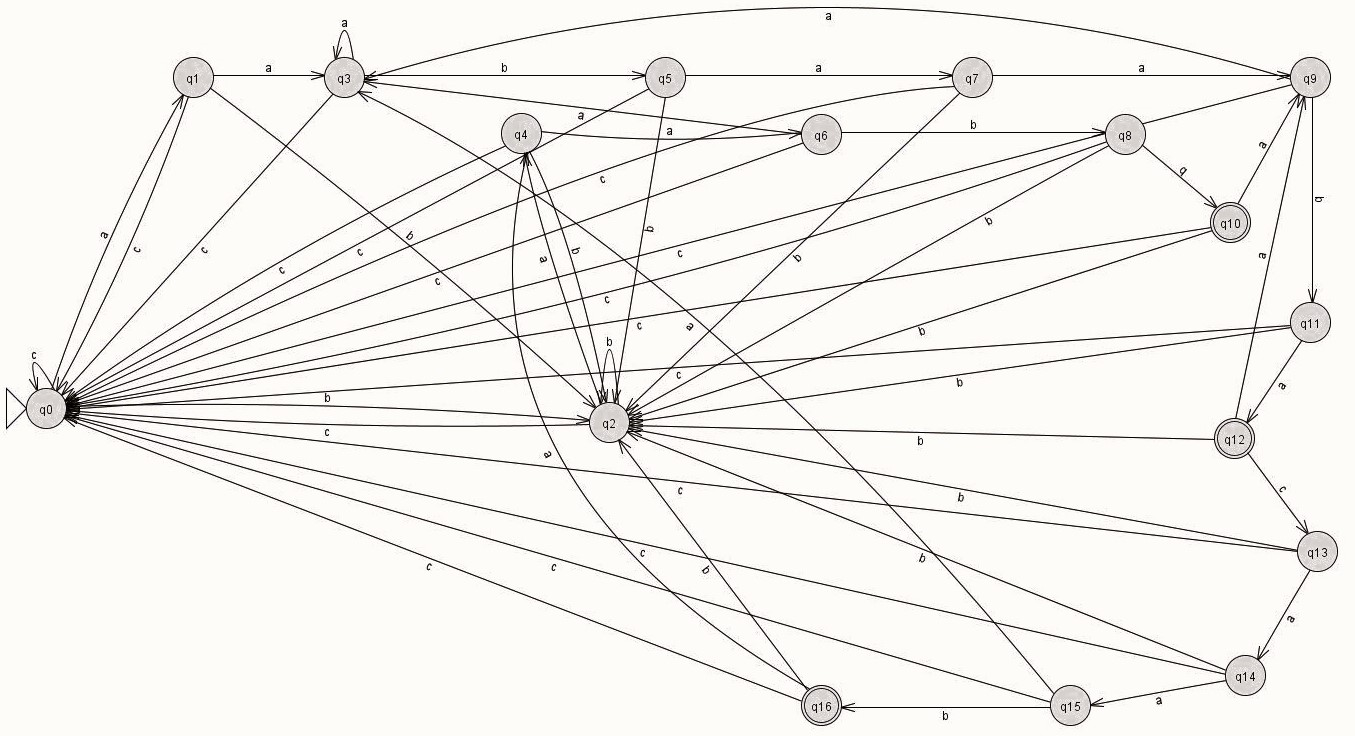
\includegraphics[width=1\linewidth]{Tarea 2 DFA 3.c.jpg}
    \captionof{figure}{DFA that accepts $w = aabaabacaab$ or $w' = baaba$ as suffix}
    \label{DFA 2}
\end{minipage}


\section{Exercise 4: \textit{Shuffle}}

For languages A and B, let the \textbf{\textit{shuffle}} of A and B the language
\begin{equation*}
    \left\{ w | w = a_1 b_1 \ldots a_k b_k , \text{ where } a_1 \ldots a_k \in A \text{ and } b_1 \ldots b_k \in B, \text{ each } a_i, b_i \in \Sigma \text{*} \right\}
\end{equation*}

Show that the class of regular languages is closed under shuffle.

\subsection{Proof}

Let $D_A = (Q_A, \Sigma, \delta_A, q_A, F_A)$ and $D_B = (Q_B, \Sigma, \delta_B, q_B, F_B)$ be two DFAs that recognize $A$ and $B$, respectively.  For this proof we need to build a NFA $N = (Q, \Sigma, \delta, q_0, F)$ that recognizes the shuffle of $A$ and $B$.

We need $N$ to track the states of $D_A$ and $D_B$. So, when we read a character, $N$ makes a move in $D_A$ and $D_B$. Also, for $N$ to accept a string it has to be $\epsilon$ or both $D_A$ and $D_B$ end in accept states. 

With this in mind, we can define $N = (Q, \Sigma, \delta, q, F)$ as follows:
\begin{enumerate}
\item $Q = (Q_A \times Q_B) \cup  \{q_0\}$, this way we can keep track of all current states of $D_A$ and $D_B$.  Also, we include the situation where nothing is read $q_0$.
\item We choose $q_0$  as the start state.
\item $F = (F_A \times F_B) \cup \{q_0\}$. This way N accepts the input only if  $D_A$ and $D_B$ accept it or if it is $\epsilon$.
\item $\delta$ can be defined as follows:
\begin{itemize}
    \item $\delta(q_0, \epsilon)=(q_A, q_B)$.
    \item $(\delta_A(x, a), y) \in \delta(x, y), a)$
    \item $(x, \delta_B(y,a)) \in \delta((x, y), a)$
\end{itemize}
\end{enumerate}
Thus, if $D_A$ is in $x$ and $D_B$ is in $y$  the state of $A$ changes according to $\delta_A=(x, a)$ and $B$ remains in $y$. In the same way, if  $D_A$ is in $x$ and $D_B$ is in $y$  the state of $B$ changes according to $\delta_B=(y, a)$ and $A$ remains in $x$.

\section{Exercise 6: \textit{Mealy machine}}

A \textbf{\textit{Mealy machine}} is a variant of a finite-state automaton that produces output; Mealy machines are sometimes called \textit{finite-state transducers}. For purposes of this problem, a Mealy machine formally consists of six components:

\begin{itemize}
    \item A finite set $\Sigma$ called the input alphabet
    \item A finite set $\Gamma$ called the output alphabet
    \item A finite set $Q$ whose elements are called states
    \item A start state $s \in Q$
    \item A transition function $\delta: Q \times \Sigma \rightarrow Q$
    \item An output function $\omega: Q \times \Sigma \rightarrow \Gamma$
\end{itemize} 

More intuitively, a Mealy machine is a graph with a special start vertex, where every node (state) has one outgoing edge labeled with each symbol from the input alphabet, and each edge (transition) is additionally labeled with a symbol from the output alphabet.

The Mealy machine reads an input string $w \in \Sigma^*$ one symbol at a time. For each symbol, the machine changes its state according to the transition function $\delta$, and simultaneously outputs a symbol according the output function $\omega$. Formally, we recursively define a transducer function $\omega^* : Q \times \Sigma^* \rightarrow \Gamma^*$ as follows:

\[
\omega^*(q,w)=
\begin{cases}
    \varepsilon & \text{if } w=\varepsilon \\
    \omega(q, a) \cdot \omega^*(\delta(q,a),x) & \text{if } w=ax, a \in \Sigma
\end{cases}
\]

Given any input string $w \in \Sigma^*$, the machine outputs the string $\omega^*(s, w) \in \Gamma^*$. To simplify notation, we define $M(w) = \omega^*(s,w)$.

Finally, the output language $L^\circ(M)$ of a Mealy machine M is the set of all strings that the machine can output:

\begin{equation*}
    L^\circ(M):=\{M(w) | w \in \Sigma \text{*} \}
\end{equation*}

\begin{enumerate}
    \item Let M be an arbitrary Mealy machine. Prove that $L^\circ(M)$ is a regular language.
    \item Let M be an arbitrary Mealy machine whose input alphabet $\Sigma$ and output alphabet $\Gamma$ are identical. Prove that the language
        \begin{equation*}
            L^= (M)=\{ w \in \Sigma^* | w = M(w)\}
        \end{equation*}
    is regular. $L^=(M)$ consists of all strings w such that M outputs w when gives input w; these are also called fixed points for the transducer function $\omega^*$.
    \item As in part (b), let M be an arbitrary Mealy machine whose input and output alphabets are identical. Prove that the language $\{ w \in \Sigma^* | w = M(M(w)) \}$ is regular.
\end{enumerate}

\subsection{Proof}

We want to prove that \(L^{\circ}(M)\) is a regular language, with \(M\) being a Mealy machine (applying the same definition as in the problem). To prove this, it is sufficient to show an automaton which recognizes \(L^{\circ}(M) = \{M(w) \, | \, w \in \Sigma^*\}\).

\textbf{Proof idea:}
At first, you would think that making any machine that receives symbols from \(\Gamma\) and reads any string from \(\Gamma^*\) could suffice. However,\textbf{ it doesn't}, because if it did, we would have to say that our new machine could read ANY set of strings, and so, making every language regular, which we know isn't true. Then, we need to construct an automaton that only reads \(L^{\circ}(M)\). In this case, let's see if we can build a finite automaton that reads a string from \(\Gamma^*\) and determines if it is a possible transduction of a string in \(\Sigma^*\) using the transduction function \(w\).

Let \(M^{\circ} = (Q^{\circ}, \Gamma, \delta^{\circ}, s_0, F^{\circ})\) be a finite automaton where:
\begin{enumerate}
    \item \(Q^{\circ} = Q\) is the set of states of \(M^{\circ}\),
    \item \(\Gamma\) is the alphabet (the same as the output alphabet of \(M\)),
    \item \(\delta^{\circ} : Q^{\circ} \times \Gamma \rightarrow Q^{\circ}\) is the transition function. We aim to read a symbol from \(\Gamma\) and determine if there exists a possible symbol in \(\Sigma\) for which the transduction yields the read symbol. To achieve this, we extend the definition as follows:
    \[
\delta^{\circ}(p, \beta) =
\begin{cases}
\emptyset, & \text{if } \beta \notin w(p, a), \text{ for any } p \in Q, a \in \Sigma \\
\{q \in Q^{\circ} \, | \, w(p, a) = \beta \land \delta(p, \beta) = q\}, & \text{if } \beta \in w(p, a), \text{ for any } p \in Q, a \in \Sigma
\end{cases}
\]

    \item \(s\) is the start state, and 
    \item \(F^{\circ} = Q^{\circ}\) is the set of accepting states of the automaton. The reason for it being equal to the set of states is that every transduction of the Mealy machine should be accepted by this new automaton.
\end{enumerate}

\textbf{Proving that M° accepts this language}

We want now to see if \(M^{\circ}\) is well-defined, that is, if \(M^{\circ}\) effectively accepts \(L^{\circ}(M)\). For this purpose, let's see if \(M(z)\), for any \(z \in \Sigma^*\), is accepted by the machine.

For the most part, it seems "obvious" that many of the elements of \(M^{\circ}\) are well-defined. For starters, \(Q^{\circ}\) is well-defined, as \(Q\) is. \(s\) is also well-defined, as it is the start state of both automata; and \(F^{\circ} = Q^{\circ}\) is well-defined due to the same reason as \(Q^{\circ}\). \(\Gamma\) is an alphabet, and then, we assume it is well-defined.

Likewise, we are missing the proof that \(\delta^{\circ}\) is well-defined. Let \(w \in \Sigma^*\) be arbitrary. Then, \(M(z) = w^*(s, z) \in \Gamma^*\) is a string in the output alphabet. For simplicity, let \(M(z) = \alpha\gamma\), for some symbol \(\alpha \in \Gamma\) and some string \(\gamma \in \Gamma^*\).

Let's compute \(\delta^{\circ}(s, M(z))\) and see if it's accepted by the automaton. 
\textbf{Proof by induction:}

\textbf{Base case:} Let \(z = \epsilon\). As \(M\) (the Mealy machine) is a definite automaton, there are no \(\epsilon\)-transitions, meaning there are no transitions for \(\epsilon\). Then, \(M(z) = M(\epsilon) = \epsilon\). This implies that \(\delta^{\circ}(s, \epsilon) = s\). \(s \in Q^{\circ}\), then \(s \in F^{\circ}\), meaning it is accepted by the automaton.

\textbf{Induction Hypothesis:} Suppose that this holds true for a string \(\gamma \in \Gamma^*\).

\textbf{Inductive step:} We want to see that this holds true for a string \(M(z) = \gamma\alpha\). \(\delta^{\circ}(s, M(z)) = \delta^{\circ}(s, \gamma\alpha)\). Following the definition of the Extended Transition Function (from the right) (assume it works for this automaton, but replace \(\delta\) with \(\delta^{\circ}\)), we can see that \(\delta^{\circ}(s, \alpha\gamma) = \delta^{\circ}(\delta^{\circ}(s, \gamma), \alpha)\). However, as \(\alpha \in \Gamma\) and it is a symbol belonging to the transduction of some string \(z\), we can safely say that \(\delta^{\circ}(p, a) \neq \emptyset\), for some \(p \in Q\). Then, \(\delta^{\circ}(s, \alpha\gamma) = \delta^{\circ}(\delta^{\circ}(s, \gamma), \alpha)\), but we know, by induction hypothesis, that \(\delta^{\circ}(s, \gamma)\) is accepted by the automaton. Then, we have a chain that is accepted by the automaton followed by a symbol that the automaton can read and will lead to a state in \(Q^{\circ}\), but any state in \(Q^{\circ}\) is an accepting state. Therefore, \(M^{\circ}\) accepts \(M(z) = \alpha\gamma\) for any \(z \in \Sigma^*\).


\subsection{Proof}

We want to prove that $L^= (M)$ is a regular language, with $M$ being a Mealy machine (applying the same definition as in the problem but changing the output alphabet to $\Sigma$). To prove this, it is sufficient to show an automaton which recognizes $L^= (M) = \{z \in \Sigma^* \mid z = M(z)\}$.

\textbf{Proof idea:} We want a machine whose language is exactly $L^= (M)$. For this, we can make an automaton that receives a string from $\Sigma^*$ and runs it through two functions: $\delta$ and $\delta(w)$. Better explained, we want a machine that reads the normal string and its transduction and decides if both are equal.

Let $M^= = \{Q^=, \Sigma, \delta^=, (s,s), F^=\}$ be a finite automaton, where:
\begin{enumerate}
    \item $Q^= = Q \times Q$ is the set of states of $M^=$ (and $Q$ is the set of states of $M$),
    \item $\Sigma$ is the alphabet,
    \item $\delta^= : Q^= \times \Sigma \rightarrow Q^=$ is the transition function. We want a transition function that reads both the input string and its transduction at the same time. We then define the function based on the following cases:
        \begin{enumerate}
            \item Case 1: If $a = \epsilon$
            \item Case 2: If $a \in \Sigma - \{\epsilon\}$ and $A = \{ \alpha \in \Sigma \mid w(q,a) = \alpha \} $
        \end{enumerate}
\[
\delta^=((p,q),a) =
\begin{cases}
    (p,q), & \text{Case 1} \\
    \{ (p',q') \mid \delta(p,a)=p' \land \delta(q,\beta)=q' \text{ for } \beta \in A \}, & \text{Case 2} 
\end{cases}
\]

    \item $(s,s)$ is the start state (with $s$ being the start state of $M$), and
    \item $F^= = \{(p,q) \in Q^= \mid p = q\}$ is the set of accepting states for $M^=$. This set of final states, and because of the nondeterminism of $M^=$, allows the machine to see if $w = M(w)$ by checking if any of the possible transductions from $w^*$ is $w$ itself, by running the resulting translation of $M(w)$ using the same transition function $\delta$.
\end{enumerate}

\textbf{Proving that $M^=$ accepts this language}
We want to see if $M^=$ is well-defined, that is, if $M^=$ effectively accepts $L^= (M)$. For this purpose, let's see if $M(z) = z$, for any $z \in \Sigma^*$, is accepted by the machine.

It may seem trivial that many of the elements of $M^=$ are well-defined. For example, $Q^=$ is well-defined, as $Q$ is. $(s,s)$ is also well-defined, as $s$ is well-defined, and $(s,s) \in Q^=$; and $F^=$ is well-defined because $Q$ is well-defined, and $F^= \cap (Q \times Q) \neq \emptyset$. $\Sigma$ is an alphabet, and then, we assume it is well-defined.

Now, we are missing the proof that $\delta^=$ is well-defined. Let $w \in \Sigma^*$ be arbitrary. Then, $M(z) = z$, and $z = xa$, for some symbol $a \in \Sigma$ and some string $x \in \Sigma^*$.

Let's compute $\delta^= ((s,s), M(z))$ and see if it's accepted by the automaton. Proof by induction:

\textbf{Base case:} Let $z = \epsilon$. As $M$ is a deterministic automaton, there are no $\epsilon$-transitions, meaning there are no transitions for $\epsilon$. Then, $M(z) = M(\epsilon) = \epsilon = z$. It is clear that $M(z) = z$. Then, we can compute $\delta^= ((s,s),a)$, but since $a = \epsilon$, then $\delta^= ((s,s),\epsilon) = (s,s)$. And $(s,s) \in F^=$, meaning the automaton clearly accepts it.

\textbf{Induction Hypothesis:} Suppose that this holds true for a string $x \in \Sigma^*$.

\textbf{Inductive step:} We want to see that this holds true for a string $M(z) = xa$. $\delta^= ((s,s), M(z)) = \delta^= ((s,s),xa)$. Following the definition of the Extended Transition Function (from the right) (assume it works for this automaton but replace $\delta$ with $\delta^=$), we can see that $\delta^= ((s,s),xa) = \delta^= (\delta^= ((s,s),x),a)$. However, by the Induction Hypothesis, we know that $\delta^= ((s,s),x)$ is accepted by the machine. But hold on, because since $a$ is part of $z$ and $M(z) = z$, then it means that for each symbol in $z$, its transduction is the same. That implies that one of the transductions of $a$ is $a$ itself. According to the definition of $\delta^=$, as there is a possible transduction of $a$, then there is a possible transition of the automaton. However, since $x$ is accepted, that means the automaton is in a state $(p,p)$ and reading $a$. But $M(a) = a$, then $\delta^= ((p,p),a) = (q,q)$ for some $q \in Q$. Then, the automaton accepts $z$.


\subsection{Proof}

We want to prove that $\{z \in \Sigma^* \mid z = M(M(z))\}$, which is similar to (b). Let $M$ be, again, a Mealy machine whose output and input alphabet are $\Sigma$, and let the rest be the same as described in the exercise.

\textbf{Proof Idea:} We need an automaton whose language is exactly that set of strings. But hold on, because this time we can retrieve a lot from (b), or better said, we can use the same automaton with some tweaks to fit our current exercise.

Let $M^= {'\hspace{0.05cm}} = \{Q^{'\hspace{0.05cm}}, \Sigma, \delta^{'\hspace{0.05cm}}, (s, s), F^{'\hspace{0.05cm}}\}$ be a finite automaton, where:
\begin{enumerate}
    \item $Q^={'} = Q \times Q$ is the set of states of $M^={'}$ (and $Q$ is the set of states of $M$),
    \item $\Sigma$ is the alphabet,
    \item $\delta^={'} : Q^={'} \times \Sigma \rightarrow Q^={'}$ is the transition function. We want a transition function that reads both the input string and the transduction of its transduction at the same time. We then define the function based on the following cases:
        \begin{enumerate}
            \item Case 1: If $a = \epsilon$
            \item Case 2: If $a \in \Sigma - \{\epsilon\}$ and $A = \{\alpha \in \Sigma \mid w(q, w(q, a)) = \alpha\} $
        \end{enumerate}
        \[
        \delta^={'}((p, q), a) =
        \begin{cases}
            (p, q), & \text{Case 1} \\
            \{ (p', q') \mid \delta(p, a) = p' \land \delta(q, \beta) = q' for \beta \in A \}, & \text{Case 2}
        \end{cases}
        \]
    \item $(s, s)$ is the start state (with $s$ being the start state of $M$), and
    \item $F^={'} = \{(p, q) \in Q^={'} \mid p = q\}$ is the set of accepting states for $M^={'}$. In the same manner as before, this set of final states allows the machine to see if $z = M(M(z))$ by checking if any of the possible transductions from $w^*(s,w^*(s, z))$ is $z$ itself, by running the resulting translation of $M(M(z))$ using the same transition function $\delta$.
\end{enumerate}

\textbf{Proving that $M^{'}$ accepts this language} 
Proving that $M^{'}$ indeed accepts this set of strings is analogous to the (b) proof, since the automaton and the languages are almost identical (you could change the set and the automaton to do an indefinite number of transductions of $z$, the result will always be $z$ since $z$ is a fixation point of $w$, the transduction function).

\pagebreak

\section{Exercise 8: \textbf{\textit{Languages derived from a regular language}}}

Let $L \subseteq \Sigma^*$ be an arbitrary regular language. Prove that the following languages are regular:

First, since $L \subseteq \Sigma^*$ is a regular language, it means that there is a finite automaton $M$ that recognizes it. Let $M = \{Q, \Sigma, \delta, q_0, F\}$ be the automaton, where:
\begin{enumerate}
    \item $Q$ is the (finite) set of states of $M$,
    \item $\Sigma$ is the (finite) alphabet of $M$,
    \item $\delta : Q \times \Sigma \rightarrow Q$ is the transition function,
    \item $q_0$ is the start state, and
    \item $F$ is the set of accepting states.
\end{enumerate}

\subsection{Proof}
Proving that $mirror(L) := \left\{ w \in \Sigma^* | ww^R \in L \right\}$ is regular.

To prove that $mirror(L) = \{w \in \Sigma^* \mid ww^R \in L\}$ is a regular language, it is, again, sufficient to show an automaton that can recognize it.

\textbf{Proof idea:} We want an automaton to which we input $w$ and it recognizes if $ww^R \in L$. For that, let's make an automaton that receives $w$ and puts it through one transition function forwards and one backwards at the same time (since the automaton can't re-read $w$), and finally see if they meet at the middle point, that is, when $M$ would've read $w$ and would start to read $w^R$.

Let $M_m = \{Q_m, \Sigma, \delta_m, s_m, F_m\}$, where:
\begin{enumerate}
    \item $Q_m = (Q \times Q) \cup \{s_m\}$ is the set of states of $M_m$,
    \item $\Sigma$ is the alphabet,
    \item $s_m$ is the start state, and
    \item $\delta_m : Q_m \times \Sigma \rightarrow Q_m$ is the transition function. We expand the definition as follows:
    
    $\delta_m (s_m, a) = \emptyset$, for any $a \in \Sigma$
    
    $\delta_m (s_m, \epsilon) = \{(q_0, f) \in Q_m \mid f \in F\}$, for $\epsilon$, the empty string
    
    $\delta_m ((p, q), a) = \{(p', q') \in Q_m \mid \delta(p, a) = p' \land \delta(q', a) = q\}$, for any $p, q \in Q$, $a \in \Sigma$

    This function assures that any string that is going to be read by the automaton will start in all states of the form $(q_0, f)$, $f \in F$, meaning that the automaton will "guess" the final state after reading $ww^R$ in $M$ and work with those states in a manner such that from $q_0$ the machine reads $w$, and from $f$ the machine reads $w^R$ backwards.
    
    \item $F_m = \{(p, q) \in Q_m \mid p = q\}$ is the set of accepting states.
\end{enumerate}

\textbf{Proving that $M_m$ does accept $mirror(L)$}

We want now to see if $M_m$ is well-defined, that is, that $M_m$ effectively accepts $mirror(L)$. For this purpose, let's see if any $z \in mirror(L)$ is accepted by the machine.

For almost all the elements, it is apparent that they are well-defined: $Q_m$ is well-defined, as $Q$ and $Q \times Q$ are. $s_m$ is also well-defined, as $s_m \in Q_m$ and there exists a transition out of $s_m$; and $F_m$ is well-defined because $Q$ is well-defined and $F_m \cap (Q \times Q) \neq \emptyset$. $\Sigma$ is an alphabet, and then, we assume it is well-defined.

We are then missing the proof that $\delta_m$ is well-defined. Let $z \in \Sigma^*$ be arbitrary such that $z \in mirror(L)$, that is, $zz^R \in L$. For simplicity, let $z = xa$, for some symbol $a \in \Sigma$ and some string $x \in \Sigma^*$.

Let's do $\delta_m (s_m, z)$ and see if it's accepted by the automaton.

\textbf{Proof by induction:}

\textbf{Base case:} Let $z = \epsilon$. First, it is clear that $\epsilon = \epsilon^R = \epsilon\epsilon^R$. Second, $\epsilon \in \Sigma$. If $\epsilon \in L$, $\epsilon\epsilon^R \in L$. Suppose that $\epsilon$ is, indeed, in $L$. Then, $\exists f' \in F$ such that $\delta(q_0, \epsilon) = f'$, and $\epsilon \in mirror(L)$. Then, there exists the pair $(f', f')$ in the transition $\delta_m (s_m, \epsilon)$, and $(f', f') \in F_m$, meaning the automaton accepts $\epsilon$.

\textbf{Induction Hypothesis:} Suppose that this holds true for a string $x \in \Sigma^*$.

\textbf{Inductive step:} Let's see that this is true for a string $z = xa$ such that $zz^R = axx^Ra \in L$. $\delta_m (s_m, z) = \delta_m (s_m, xa)$. Following the definition of the Extended Transition Function (from the left) (assume it works for this automaton but replace $\delta$ for $\delta_m$), we can see that $\delta_m (s_m, ax) = \delta_m (\delta_m (s_m, \varepsilon a), x)$. From the definition of $\delta_m$, 

$\delta_m (s_m, \epsilon a) = \{(p', f) \in Q_m \mid \delta(\delta(q_0, a), x) = p' \land \exists z \in \Sigma^* \text{ such that } |z| = 2^{1+|x|} \land \delta^*(p', z) = f \in F\}$. Since $axx^Ra \in L$, there are three states $q_a$, $r_x$, $p_a$ such that $\delta(q_0, a) = q_a$, $\delta(q_a, x) = r_x$, $\delta(r_x, x^R) = p_a$, $\delta(p_a, a) = f \in F$. However, $(q_a, p_a) \in \delta_m (s_m, \epsilon a)$. And, from Induction Hypothesis, it is true to say that $\delta_m ((q_a, p_a), x)$ contains an ordered pair of the form $(r_x, r_x) \in F_m$. Then, $z$ is accepted by the automaton.

\subsection{Proof}
Proving that $log(L) := \left\{ x \in \Sigma^* | xy \in l \text{ for some } y \in \Sigma^* \text{ such that } |y|=2^{|x|} \right\} $ is regular. 

To prove that $\log(L) = \{x \in \Sigma^* \mid \exists y \in \Sigma^* \text{ such that } |y| = 2^{|x|} \land xy \in L\}$ is a regular language, it is sufficient to show an automaton that can recognize it.

\textbf{Proof Idea:} We want an automaton that specifically accepts strings of length $n$ for which there exists a string of a specific length $2^n$ leading to an accepting state. Let's try to make an automaton that captures that idea.

Let $M_{\text{log}} = \{Q_{\text{log}}, \Sigma, \delta_{\text{log}}, s_{\text{log}}, F_{\text{log}}\}$, where:
\begin{enumerate}
    \item $Q_{\text{log}} = (Q \times Q) \cup \{s_{\text{log}}\}$ is the set of states of $M_{\text{log}}$,
    \item $\Sigma$ is the alphabet,
    \item $s_{\text{log}}$ is the start state, and
    \item $\delta_{\text{log}} : Q_{\text{log}} \times \Sigma \rightarrow Q_{\text{log}}$ is the transition function. We clarify the definition as follows:
    
    $\delta_{\text{log}} (s_{\text{log}}, a) = \emptyset$, for any $a \in \Sigma$
    
    $\delta_{\text{log}} (s_{\text{log}}, \epsilon) = \{(q_0, q) \in Q_m \mid \exists a \in \Sigma \text{ such that } \delta(q_0, a) = q\}$, for $\epsilon$
    
    For any $p, q \in Q$, $a \in \Sigma$:
    
    $\delta_{\text{log}} ((p, q), a) = \{(p', q') \in Q_m \mid \delta(p, a) = p' \land \exists z \in \Sigma^* \text{ such that } |z| = 2 \land \delta^*(p', z) = q'\}$
    
    Extending the function to any string: For any $p, q \in Q$, $w \in \Sigma^*$, supposing that $w = ax$:
    
    $\delta_{\text{log}} ((p, q), w) = \{(p', f) \in Q_m \mid \delta^*(\delta(p, a), x) = p' \land \exists z \in \Sigma^* \text{ such that } |z| = 2^{1+|x|} \land \delta^*(p', z) = f \in F\}$

    We are defining a function that "captures the essence" of the language, that is, that it exactly does what it needs to do: Verify if there is a string of length $2^|w|$ that can take the read string from its actual state to an accepting one. If there is, then it will be accepted, if it isn't, then it will not. 
    
    \item $F_{\text{log}} = \{(q, f) \in Q_m \mid q \in Q \land f \in F\}$ is the set of accepting states.
\end{enumerate}

\textbf{(Proving that $M_{\text{log}}$ does accept $\log(L)$):}

Now, we try and see if $M_{\text{log}}$ is well-defined, that is, that it effectively accepts this language it was designed for. Let's see if $z \in \log(L)$ is accepted by $M_{\text{log}}$.

Again, it is apparent that many of the elements of the automaton are well-defined. To start, $Q_{\text{log}}$ is well-defined, as $Q$ and $Q \times Q$ are. $s_{\text{log}}$ is also well-defined, as $s_{\text{log}} \in Q_{\text{log}}$ and there is a transition going out of $s_{\text{log}}$; and $F_{\text{log}}$ is well-defined too, as $Q$ and $F$ are well-defined. $\Sigma$ is an alphabet, and then, we assume it is well-defined.

Like so, we are missing the proof that $\delta_{\text{log}}$ is well-defined. Let $z \in \log(L)$. For simplicity, let $z = ax$, for some symbol $a \in \Sigma$ and some string $x \in \Sigma^*$.

Let's do $\delta_{\text{log}} (s_{\text{log}}, z)$ and see if it's accepted by the automaton.

\textbf{Proof by induction:}

\textbf{Base case:} Let $z = \epsilon$. As we assumed that $\epsilon = z \in \log(L)$, then $zy \in L$ for some $y \in \Sigma^*$ such that $|y| = 2^{|z|} = 2^0 = 1$. For that reason, $\exists f_y \in F$ such that $\delta(q_0, y) = f_y$. From the definition of $\delta_{\text{log}}$, $\delta_{\text{log}} (s_{\text{log}}, \epsilon) = \{(q_0, q) \in Q_{\text{log}} \mid \exists a \in \Sigma \text{ such that } \delta(q_0, a) = q\}$. That set is not empty, as $(q_0, f_y)$ is effectively in it, and $(q_0, f_y) \in F_{\text{log}}$. Then, $M_{\text{log}}$ accepts $z$.

\textbf{Induction Hypothesis:} Suppose that this holds true for a string $x = bk \in \Sigma^*$.

\textbf{Inductive step:} We want to see that this is true for a string $z = ax$. $\delta_{\text{log}} (s_{\text{log}}, z) = \delta_{\text{log}} (s_{\text{log}}, ax)$. As we say that $z \in \log(L)$, then $zy \in L$ for some $y \in \Sigma^*$ such that $|y| = 2^{|x|}$ and $\delta_{\text{log}} ((q_0, q), x) = \{(p', f) \in Q_{\text{log}} \mid \delta^*(\delta(q_0, b), k) = p' \land \exists y' \in \Sigma^* \text{ such that } |y'| = 2^{|x|} \land \delta^*(p', y') = f \in F\}$.

Then, we can apply an inductive definition on the previous function, giving us that:

$\delta_{\text{log}} ((q_0, q), z) = \{(p', f) \in Q_{\text{log}} \mid \delta^*(\delta(q_0, a), x) = p' \land \exists y \in \Sigma^* \text{ such that } |y| = 2^{1+|x|} \land \delta^*(p', y) = f \in F\}$, which is a non-empty set since $z \in \log(L)$ (which implies that there exists a $y$).

Then $M_{\text{log}}$ accepts $z$.
    
\end{document}